\documentclass[tikz,border=10pt]{standalone}
\usepackage[T1]{fontenc}
\usepackage[utf8]{inputenc}
\usepackage{lmodern}
\usepackage{amsmath,amssymb}
\usetikzlibrary{arrows.meta,positioning,shapes.geometric,calc}
\definecolor{jac}{HTML}{73539E}
\definecolor{ink}{HTML}{354052}
\tikzset{
 >=Stealth,
 state/.style={draw=jac,fill=jac!7,rounded corners=5pt,align=center,minimum width=26mm,minimum height=11mm,inner sep=5pt,font=\small},
 action/.style={state,fill=white},
 decision/.style={draw=jac,fill=jac!7,diamond,aspect=2.4,inner sep=1.8pt,align=center,font=\small},
 success/.style={state,draw=teal!75!black,fill=teal!7},
 failure/.style={state,draw=red!70!black,fill=red!5},
 arrow/.style={->,thick,draw=ink},
 note/.style={align=left,font=\footnotesize,text=ink}
}
\begin{document}

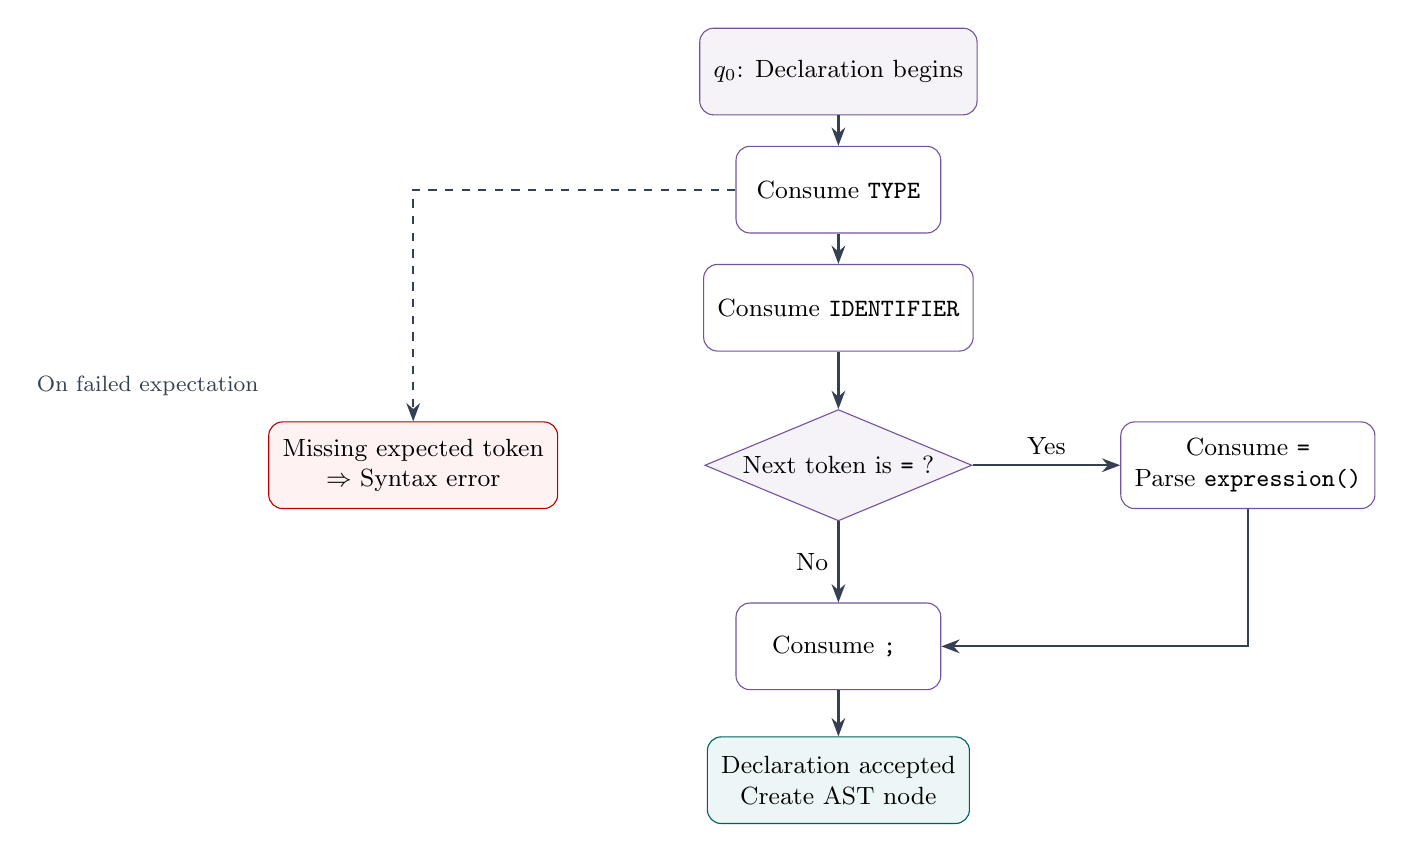
\begin{tikzpicture}[font=\small]
\node[state] (q0) at (0,0) {$q_0$: Declaration begins};
\node[action] (q1) at (0,-1.5) {Consume \texttt{TYPE}};
\node[action] (q2) at (0,-3) {Consume \texttt{IDENTIFIER}};
\node[decision] (d) at (0,-5) {Next token is \texttt{=} ?};
\node[action] (e) at (5.2,-5) {Consume \texttt{=}\\Parse \texttt{expression()}};
\node[action] (q3) at (0,-7.3) {Consume \texttt{;} };
\node[success] (q4) at (0,-9) {Declaration accepted\\Create AST node};
\node[failure] (err) at (-5.4,-5) {Missing expected token\\$\Rightarrow$ Syntax error};
\draw[arrow] (q0)--(q1);\draw[arrow] (q1)--(q2);\draw[arrow] (q2)--(d);
\draw[arrow] (d)--node[left]{No}(q3);
\draw[arrow] (d)--node[above]{Yes}(e);
\draw[arrow] (e) |- (q3);
\draw[arrow] (q3)--(q4);
\draw[arrow,dashed] (q1.west) -| (err.north);
\node[note,above left=2mm and 0mm of err] {On failed expectation};
\end{tikzpicture}

\end{document}
